\documentclass[11pt,a4paper]{article}

% -----------------------------------------------------------------------
% Packages (minimal set to avoid font issues)
% -----------------------------------------------------------------------
\usepackage[margin=1in]{geometry}
\usepackage[T1]{fontenc}
\usepackage{lmodern}
\usepackage{amsmath,amssymb}
\usepackage{booktabs}
\usepackage{graphicx}
\usepackage{enumitem}
\usepackage{parskip}

% -----------------------------------------------------------------------
% Title
% -----------------------------------------------------------------------
\title{%
  \textbf{AutoRAGEvals: A Self-Improving Loop for RAG Pipeline Optimization}\\[0.5em]
  \large Using Claude as a Meta-Optimizer with RAGAS and ROUGE-L Evaluation
}

\author{%
  Yegan Metz\\
  \textit{Independent Research}
}

\date{May 2026}

% -----------------------------------------------------------------------
\begin{document}

\maketitle

% -----------------------------------------------------------------------
\begin{abstract}
% -----------------------------------------------------------------------
We present \textbf{AutoRAGEvals}, an automated framework that iteratively
optimizes a Retrieval-Augmented Generation (RAG) pipeline without human
intervention. The system uses Claude as a meta-optimizer: it reads the current
pipeline configuration and RAGAS evaluation scores, then proposes a single
hyperparameter change per iteration. Each proposed configuration is evaluated
three times (mean $\pm$ std reported) using RAGAS faithfulness, answer
relevancy, context precision, context recall, and ROUGE-L. Changes that improve
the mean overall score are kept; others are reverted. Over eight optimizer
iterations on 38 adversarial questions, the framework raises the overall RAGAS
score from 0.7019 (baseline, \texttt{top\_k}=3) to 0.7807 (best, \texttt{top\_k}=7),
a gain of $+7.9$ percentage points. All gains come from increasing retrieval
breadth (\texttt{top\_k}); all chunking and prompt-variant changes revert.
Held-out evaluation on 50 unseen HotpotQA questions reveals a large
generalization gap (0.3439 vs.\ 0.7807), driven by low corpus coverage rather
than model error. We further demonstrate that ROUGE-L and RAGAS can diverge in
opposite directions, making the choice of evaluation metric consequential for
optimization decisions.
\end{abstract}

% -----------------------------------------------------------------------
\section{Introduction}
% -----------------------------------------------------------------------

Retrieval-Augmented Generation (RAG) pipelines are sensitive to numerous
hyperparameters: document chunking strategy, retrieval breadth, prompt
formulation, and optional reranking. Tuning these parameters typically requires
substantial human effort---practitioners manually inspect outputs, hypothesize
changes, and re-evaluate. This cycle is slow, costly, and difficult to
reproduce.

We propose \textbf{AutoRAGEvals}, a closed optimization loop that automates
this process entirely. The key insight is that a capable language model
(Claude) can serve simultaneously as a \emph{meta-optimizer}---reading
evaluation scores and proposing principled hyperparameter changes---and as a
\emph{question generator}---creating challenging adversarial questions that
stress-test the pipeline.

The framework is inspired by Karpathy's \texttt{autoresearch} concept of
self-improving loops and extends it with: (1) multi-metric RAG evaluation via
RAGAS~\cite{es2023ragas}; (2) statistical robustness through multi-run scoring;
(3) a held-out generalization evaluation; and (4) publication-quality
visualization of the optimization trajectory.

\textbf{Key contributions:}
\begin{itemize}[leftmargin=2em]
  \item A fully automated, resumable RAG hyperparameter optimizer requiring no
    human intervention.
  \item An adversarial question set (50 questions: multi-hop, ambiguous,
    out-of-scope, paraphrase) generated by Claude for rigorous evaluation.
  \item Empirical evidence that retrieval breadth (\texttt{top\_k}) is the
    dominant lever for HotpotQA multi-hop questions, while chunking and
    prompt-variant changes provide no benefit.
  \item Demonstration of the ROUGE-L vs.\ RAGAS metric divergence phenomenon
    and its practical implications.
  \item Analysis of a large in-distribution vs.\ held-out generalization gap
    caused by corpus coverage constraints.
\end{itemize}

% -----------------------------------------------------------------------
\section{Background and Related Work}
% -----------------------------------------------------------------------

\subsection{Retrieval-Augmented Generation}

RAG~\cite{lewis2020rag} combines a retrieval component (vector similarity
search) with a generative language model. Given a query, the retriever fetches
relevant document chunks; the generator synthesizes an answer conditioned on
both the query and retrieved context. Key hyperparameters include chunk size,
chunk overlap, the number of retrieved chunks ($k$), the prompt template, and
optional reranking.

\subsection{RAGAS Evaluation}

RAGAS~\cite{es2023ragas} provides four LLM-based metrics without requiring
human reference answers for some dimensions:
\begin{description}[leftmargin=2em]
  \item[Faithfulness] --- fraction of answer claims that are grounded in the
    retrieved context (0--1).
  \item[Answer Relevancy] --- cosine similarity between the generated answer and
    the original question (embedding-based).
  \item[Context Precision] --- proportion of retrieved chunks that are relevant
    to the gold answer.
  \item[Context Recall] --- proportion of gold-answer claims that can be
    attributed to the retrieved context.
\end{description}
We also track \textbf{ROUGE-L}~\cite{lin2004rouge} as a surface-level lexical
overlap metric between the generated answer and the gold answer string.

\subsection{HotpotQA}

HotpotQA~\cite{yang2018hotpotqa} is a multi-hop question answering dataset
requiring reasoning across multiple Wikipedia passages. We use the distractor
dev split (7,405 questions) as our corpus source and optimization benchmark.
Due to computational constraints, we index only 300 passages, which creates a
retrieval coverage ceiling discussed in Section~\ref{sec:findings}.

\subsection{Meta-Optimization with LLMs}

Recent work uses LLMs to optimize prompts and hyperparameters. AutoRAGEvals
applies this paradigm to the full RAG pipeline, proposing changes one parameter
at a time and using objective scores to accept or reject changes---analogous
to coordinate descent with stochastic evaluation.

% -----------------------------------------------------------------------
\section{System Architecture}
% -----------------------------------------------------------------------

Figure~\ref{fig:architecture} illustrates the optimization loop. Claude
proposes one hyperparameter change per iteration; RAGAS + ROUGE-L evaluate the
result; the loop keeps or reverts based on the mean overall RAGAS score across
three runs.

\begin{figure}[ht]
\centering
\begin{verbatim}
+----------------------------------------------------------+
|                   AutoRAGEvals Loop                      |
|                                                          |
|  Document Corpus (HotpotQA dev)                          |
|       |                                                  |
|       v                                                  |
|  +----------+   chunk_size, chunk_overlap,  +---------+  |
|  | RAG      |   top_k, prompt_variant,      | Claude  |  |
|  | Pipeline |<-- reranker                   |Optimizer|  |
|  |(LlamaIndex|                              +---------+  |
|  |+ChromaDB)|                                   |        |
|  +----+-----+                           propose next     |
|       |                                 param change     |
|       | answers + contexts                    |          |
|       v                                       |          |
|  +----------+   scores               +--------+------+   |
|  |  RAGAS   |----------------------->|  Keep / Revert|   |
|  |  Scorer  |                       +---------------+   |
|  | +ROUGE-L |                                           |
|  +----------+                                           |
|                                                          |
|  Each config scored 3x -> mean +/- std reported         |
|  Best config persisted across iterations (resumable)    |
+----------------------------------------------------------+
\end{verbatim}
\caption{AutoRAGEvals optimization loop.}
\label{fig:architecture}
\end{figure}

\subsection{RAG Pipeline}

The pipeline is implemented with LlamaIndex 0.10 and ChromaDB 0.5 as the
vector store. Documents are embedded with OpenAI \texttt{text-embedding-3-small}
and answers are generated with \texttt{gpt-4o-mini}. Three prompt templates
are available: \texttt{baseline} (standard context-then-query),
\texttt{concise} (1--2 sentence response), and \texttt{chain\_of\_thought}
(step-by-step reasoning before answer). An optional reranker uses
\texttt{CohereRerank} if \texttt{COHERE\_API\_KEY} is set, otherwise falls
back to \texttt{LLMRerank}.

\subsection{Claude Optimizer}

At each iteration, Claude receives: (1) the current hyperparameter
configuration, (2) all RAGAS and ROUGE-L scores (mean $\pm$ std), and (3)
the full history of past proposals and keep/revert decisions. It responds with
a structured JSON object specifying one parameter to change, the old value,
the new value, and a one-sentence rationale. The keep/revert decision is made
purely on the mean overall RAGAS score relative to the current best.

\subsection{Statistical Robustness}

Each proposed configuration is evaluated $N=3$ times. The RAG index is built
once (deterministic); query and scoring passes run three times to capture
variance from LLM temperature sampling. We report mean $\pm$ std for all
metrics. The standard deviation is stored in the log and serves as a
confidence indicator.

\subsection{Search Space}

\begin{table}[ht]
\centering
\caption{Hyperparameter search space explored by the optimizer.}
\label{tab:search_space}
\begin{tabular}{lll}
\toprule
\textbf{Parameter} & \textbf{Values} & \textbf{Default} \\
\midrule
\texttt{chunk\_size}     & 256, 512, 1024 & 512 \\
\texttt{chunk\_overlap}  & 25, 50, 100    & 50  \\
\texttt{top\_k}          & 3, 5, 7        & 3   \\
\texttt{prompt\_variant} & baseline, concise, chain\_of\_thought & baseline \\
\texttt{reranker}        & True, False    & False \\
\bottomrule
\end{tabular}
\end{table}

% -----------------------------------------------------------------------
\section{Experimental Setup}
% -----------------------------------------------------------------------

\subsection{Data}

\textbf{Corpus.} We load 300 passages from the HotpotQA distractor dev set
using the HuggingFace \texttt{datasets} library (validation split). Passages
are deduplicated by exact text match, yielding 2,964 unique document chunks
after ingestion with the default chunk\_size=512, chunk\_overlap=50.

\textbf{Adversarial questions.} We use Claude (\texttt{claude-sonnet-4-20250514})
to generate 50 adversarial questions from the indexed passages, covering four
categories: multi-hop (14), ambiguous (12), out-of-scope (12), and paraphrase
(12). Of these, 38 are scoreable by RAGAS; the 12 out-of-scope questions have
no supporting context and are excluded from optimization scoring.

\textbf{Held-out questions.} We randomly sample 50 questions from the HotpotQA
dev set (seed=42), filtering out questions appearing in the adversarial set and
yes/no questions. These are never seen during optimization and serve as a
generalization test.

\subsection{Metrics}

The primary optimization signal is \textbf{overall RAGAS}, computed as the
arithmetic mean of faithfulness, answer relevancy, context precision, and
context recall. ROUGE-L is tracked as a secondary monitor-only metric and does
not influence keep/revert decisions.

\subsection{Reproducibility}

The optimizer is fully resumable via \texttt{experiment\_log.json}. On restart,
it reads the last kept configuration and continues from the next iteration.
API calls use default temperature settings; the three-run mean reduces
sensitivity to individual sampling outcomes.

% -----------------------------------------------------------------------
\section{Results}
% -----------------------------------------------------------------------

\subsection{Optimization Trajectory}

Table~\ref{tab:trajectory} shows the full optimization trajectory on the 38
adversarial questions.

\begin{table}[ht]
\centering
\caption{Optimizer iteration scores (adversarial set, 38 questions).
Overall RAGAS = mean of faithfulness, answer relevancy, context precision,
context recall. Iterations 6--7 show mean $\pm$ std across 3 runs.}
\label{tab:trajectory}
\begin{tabular}{clccl}
\toprule
\textbf{Iter} & \textbf{Change} & \textbf{Overall RAGAS} & \textbf{$\Delta$} & \textbf{Decision} \\
\midrule
0 & Baseline (\texttt{top\_k}=3)           & 0.7019              & ---     & Kept \\
1 & \texttt{top\_k}: 3$\to$5              & 0.7475              & +0.0456 & Kept \\
2 & \texttt{top\_k}: 5$\to$7              & 0.7807              & +0.0332 & \textbf{Kept (best)} \\
3 & \texttt{chunk\_overlap}: 50$\to$100   & 0.7581              & $-$0.0226 & Reverted \\
4 & \texttt{chunk\_overlap}: 50$\to$25    & 0.7386              & $-$0.0421 & Reverted \\
5 & \texttt{chunk\_size}: 512$\to$1024    & 0.7380              & $-$0.0427 & Reverted \\
6 & \texttt{prompt\_variant}: chain\_of\_thought & $0.7368 \pm 0.013$ & $-$0.0439 & Reverted \\
7 & \texttt{prompt\_variant}: concise     & $0.7434 \pm 0.011$ & $-$0.0373 & Reverted \\
\bottomrule
\end{tabular}
\end{table}

Figure~\ref{fig:iteration_scores} plots the trajectory. Green dots indicate
kept configurations; red dots indicate reverted configurations. Error bars
appear at iterations 6--7 where multi-run scoring was first applied.

\begin{figure}[ht]
\centering
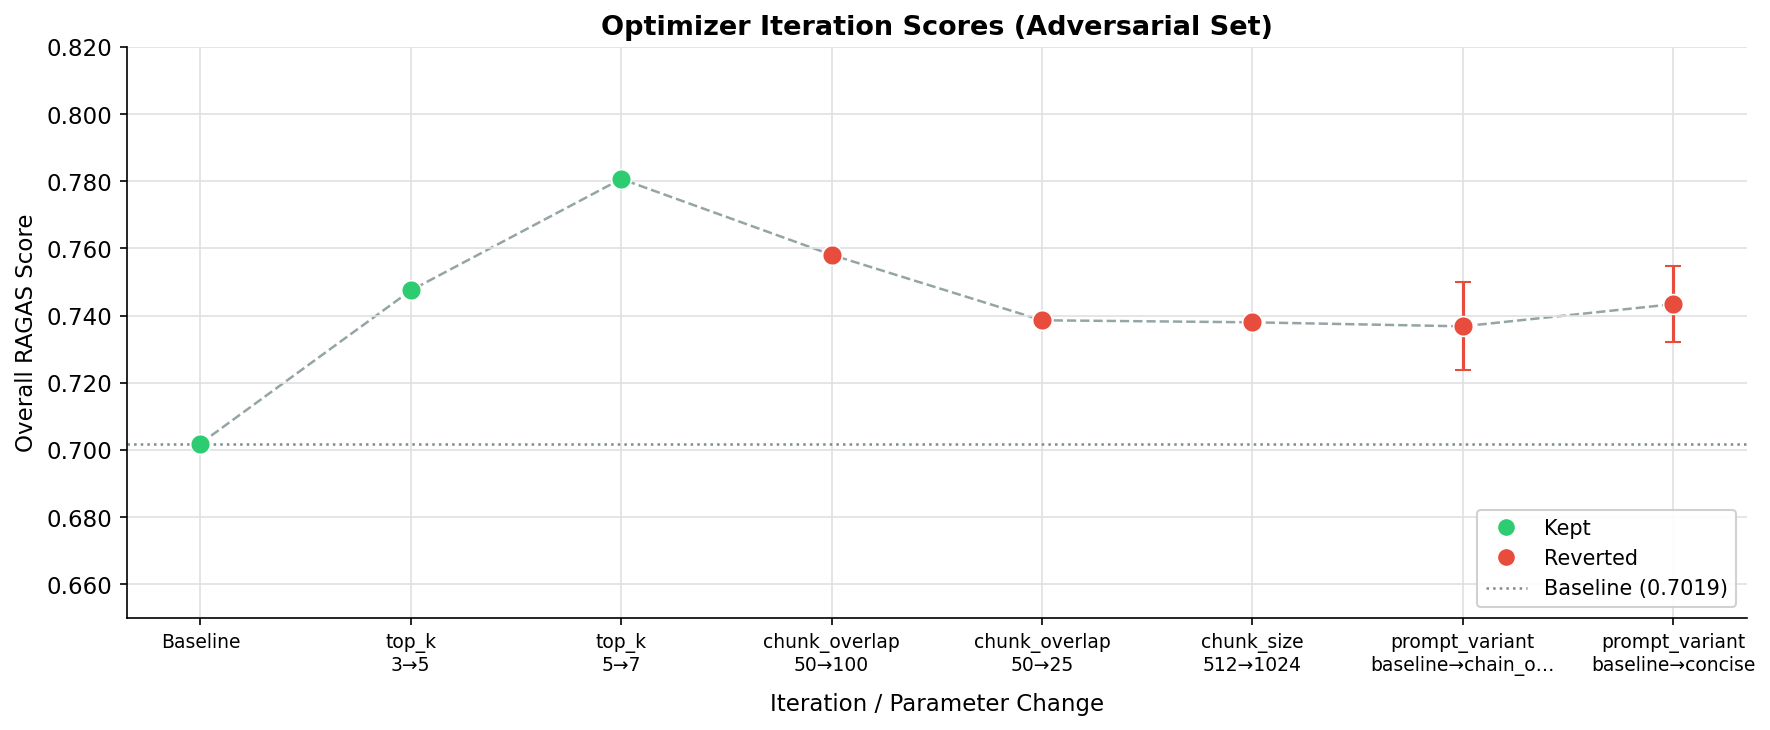
\includegraphics[width=\textwidth]{figures/fig1_iteration_scores.png}
\caption{Overall RAGAS score across all 8 optimizer iterations. Green markers
= kept (improvement); red markers = reverted (regression). Error bars show
$\pm$1 std across 3 evaluation runs (iters 6--7). The dashed line marks the
baseline at 0.7019.}
\label{fig:iteration_scores}
\end{figure}

\subsection{Per-Metric Comparison}

Table~\ref{tab:per_metric_adv} and Figure~\ref{fig:per_metric_bars} compare
baseline and best configurations across all five metrics on the adversarial set.

\begin{table}[ht]
\centering
\caption{Baseline vs.\ best configuration --- per-metric scores on the
adversarial evaluation set (38 questions).}
\label{tab:per_metric_adv}
\begin{tabular}{lccc}
\toprule
\textbf{Metric} & \textbf{Baseline (\texttt{top\_k}=3)} & \textbf{Best (\texttt{top\_k}=7)} & \textbf{$\Delta$} \\
\midrule
Faithfulness        & 0.8377 & 0.9057 & +0.068 \\
Answer Relevancy    & 0.7683 & 0.8034 & +0.035 \\
Context Precision   & 0.5614 & 0.6376 & +0.076 \\
Context Recall      & 0.6404 & 0.7763 & +0.136 \\
\textbf{Overall}    & \textbf{0.7019} & \textbf{0.7807} & \textbf{+0.079} \\
ROUGE-L             & 0.1449 & 0.1596 & +0.015 \\
\bottomrule
\end{tabular}
\end{table}

\begin{figure}[ht]
\centering
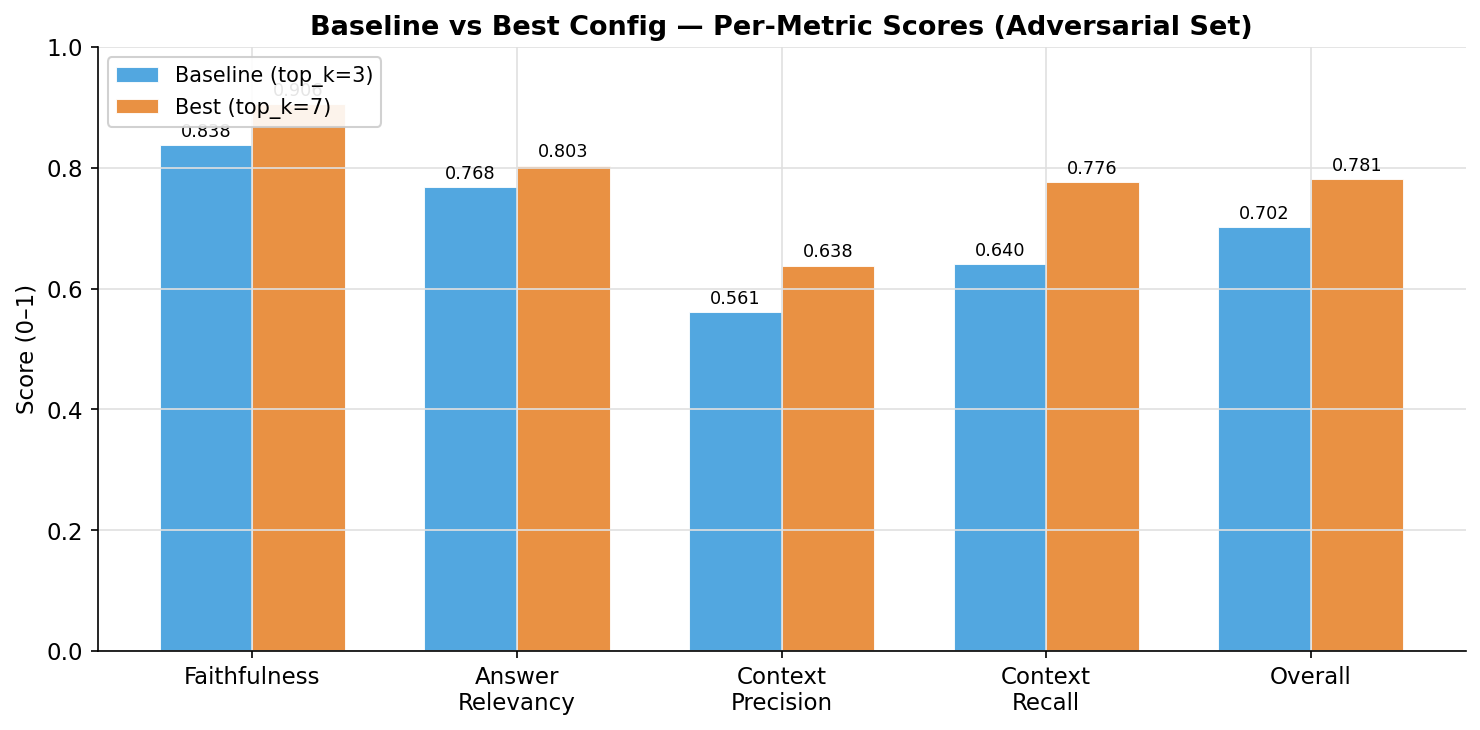
\includegraphics[width=0.9\textwidth]{figures/fig2_per_metric_bars.png}
\caption{Grouped bar chart: baseline (blue) vs.\ best (orange) across all five
RAGAS metrics on the adversarial evaluation set. All five metrics improve under
the best configuration; context recall shows the largest gain (+0.136).}
\label{fig:per_metric_bars}
\end{figure}

The largest individual gain is in \textbf{context recall} (+0.136), which
measures how much of the gold answer's factual content is covered by retrieved
chunks. Increasing $k$ from 3 to 7 retrieves more supporting passages,
directly raising recall. Context precision also improves (+0.076), suggesting
that the additional chunks are predominantly relevant for these adversarial
questions.

\subsection{Held-Out Generalization Evaluation}

Table~\ref{tab:per_metric_ho} and Figure~\ref{fig:generalization} show scores
on the 50 held-out HotpotQA questions never seen during optimization.

\begin{table}[ht]
\centering
\caption{Baseline vs.\ best configuration --- all metrics on both evaluation sets.}
\label{tab:per_metric_ho}
\begin{tabular}{lcccccc}
\toprule
 & \multicolumn{3}{c}{\textbf{Adversarial Set}} & \multicolumn{3}{c}{\textbf{Held-out Set}} \\
\cmidrule(lr){2-4}\cmidrule(lr){5-7}
\textbf{Metric} & Base & Best & $\Delta$ & Base & Best & $\Delta$ \\
\midrule
Faithfulness      & 0.8377 & 0.9057 & +0.068 & 0.3767 & 0.4691 & +0.092 \\
Answer Relevancy  & 0.7683 & 0.8034 & +0.035 & 0.6380 & 0.6064 & $-$0.032 \\
Context Precision & 0.5614 & 0.6376 & +0.076 & 0.1600 & 0.1600 & +0.000 \\
Context Recall    & 0.6404 & 0.7763 & +0.136 & 0.1200 & 0.1400 & +0.020 \\
\textbf{Overall}  & \textbf{0.7019} & \textbf{0.7807} & \textbf{+0.079} & \textbf{0.3237} & \textbf{0.3439} & \textbf{+0.020} \\
ROUGE-L           & 0.1449 & 0.1596 & +0.015 & 0.0901 & 0.0838 & $-$0.006 \\
\bottomrule
\end{tabular}
\end{table}

\begin{figure}[ht]
\centering
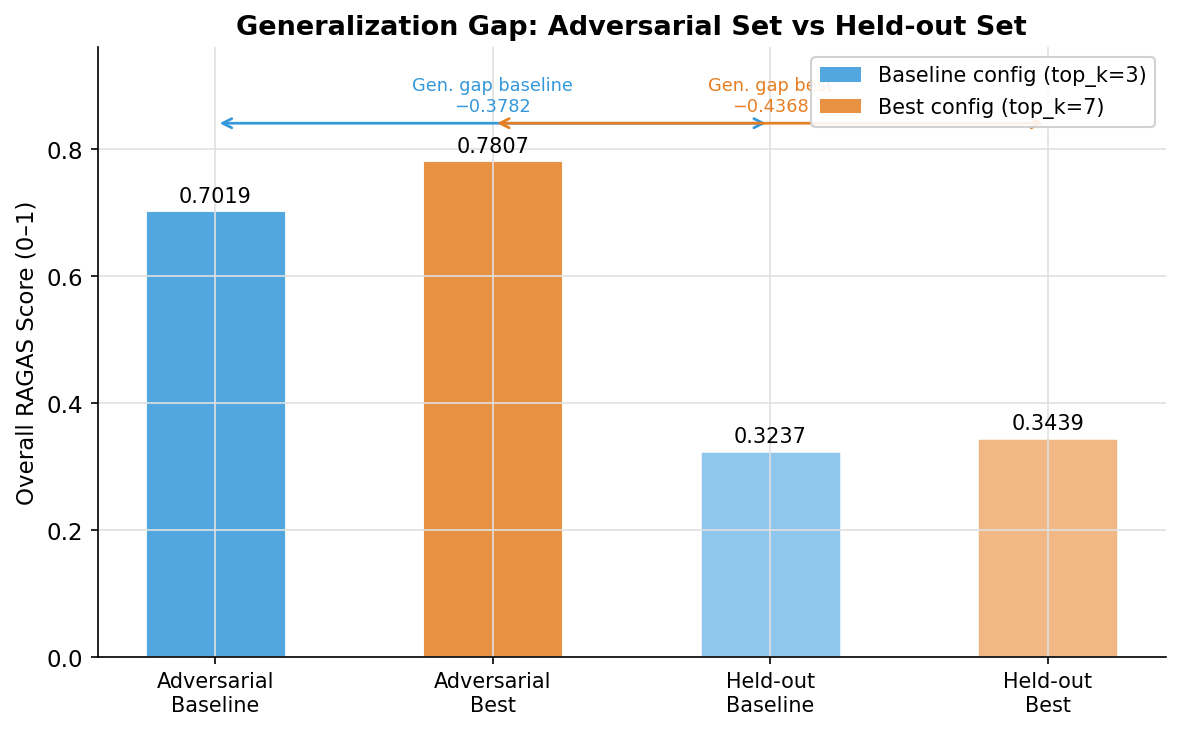
\includegraphics[width=0.85\textwidth]{figures/fig3_generalization.png}
\caption{Generalization gap between the adversarial evaluation set and the
held-out HotpotQA set. Both baseline and best configs score dramatically lower
on held-out questions ($\approx$0.34 vs.\ $\approx$0.78), driven by low
retrieval coverage: only 300 of 7,405 HotpotQA passages are indexed.}
\label{fig:generalization}
\end{figure}

The held-out overall RAGAS score (0.3439) is 0.437 below the adversarial best
(0.7807). This large generalization gap is analyzed in
Section~\ref{sec:findings}.

\subsection{ROUGE-L vs.\ RAGAS Divergence}

Figure~\ref{fig:rouge_vs_ragas} plots both RAGAS overall and ROUGE-L across
all 8 iterations on a dual y-axis.

\begin{figure}[ht]
\centering
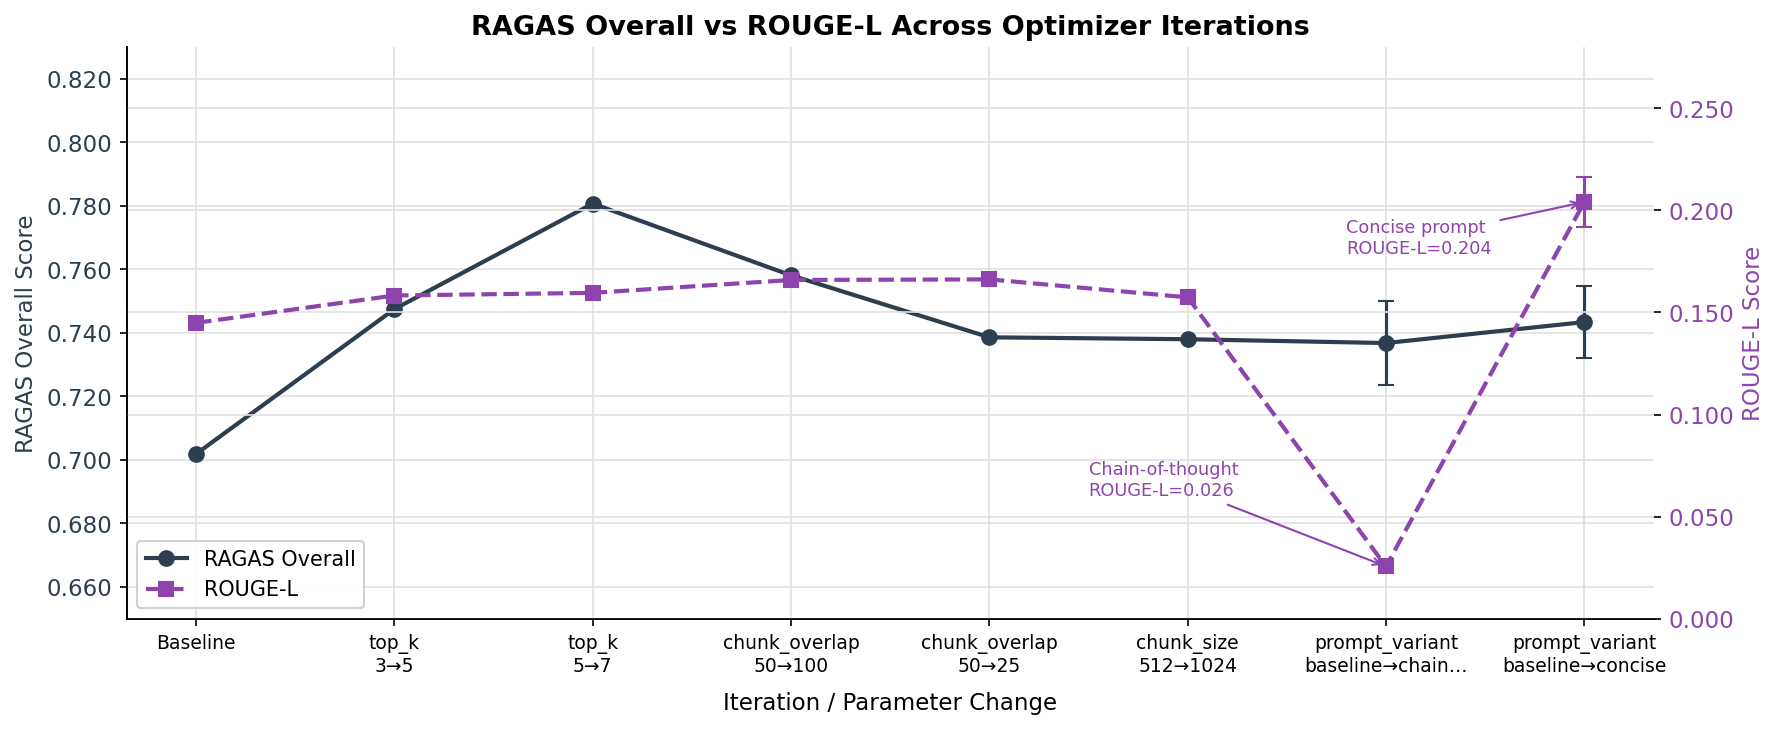
\includegraphics[width=\textwidth]{figures/fig4_rouge_vs_ragas.png}
\caption{RAGAS overall (dark navy, left axis) and ROUGE-L (purple dashed, right
axis) across all 8 optimizer iterations. At iteration 7 (concise prompt),
ROUGE-L spikes to 0.204 while RAGAS overall falls to 0.743. At iteration 6
(chain-of-thought), ROUGE-L collapses to 0.026 while RAGAS overall falls to
0.737.}
\label{fig:rouge_vs_ragas}
\end{figure}

The most striking divergence occurs at iteration 7 (\texttt{concise} prompt):
ROUGE-L rises from 0.160 (iter 2 best) to 0.204, while RAGAS overall falls
from 0.781 to 0.743. The concise prompt produces shorter, more lexically
aligned answers (higher ROUGE-L) at the cost of lower faithfulness and
completeness (lower RAGAS). Chain-of-thought (iteration 6) shows the opposite:
ROUGE-L collapses to 0.026 while RAGAS falls only moderately.

% -----------------------------------------------------------------------
\section{Case Studies}
\label{sec:case_studies}
% -----------------------------------------------------------------------

We select three illustrative questions from the held-out set to show how
pipeline behavior changes between baseline and best configurations.

\subsection{Case 1: Improved Answer}

\textbf{Question:} \emph{``What is the name the Colombian film loosely based on
a story about a dying child's dreams and hope first published in 1845 by Hans
Christian Andersen?''}

\textbf{Gold answer:} \emph{The Little Match Girl}

The baseline (\texttt{top\_k}=3) retrieved three chunks about Andersen fairy
tales but not the passage containing the film title, and hallucinated
``La ni\~na de la mochila azul'' (ROUGE-L = 0.051). The best config
(\texttt{top\_k}=7) retrieved four additional chunks, one of which contained
the correct title, and produced the correct answer (ROUGE-L = 0.222,
$\Delta = +0.171$). This illustrates the primary mechanism of top-k improvement:
broader retrieval increases the probability of including the supporting passage.

\subsection{Case 2: Retrieval Coverage Failure}

\textbf{Question:} \emph{``In what century did this Native warrior and chief,
whose brother Tenskwatawa led the Tippecanoe order of battle, become the primary
leader of a large, multi-tribal confederacy?''}

\textbf{Gold answer:} \emph{nineteenth}

Both configurations retrieve passages about Tecumseh's confederacy and the
Battle of Tippecanoe but neither produces the bare token ``nineteenth'' as
required. Both answer ``early 19th century'' (ROUGE-L = 0.000 for both). The
correct supporting passage is not among the 300 indexed documents---this is a
corpus coverage failure, not a generation failure. Increasing \texttt{top\_k}
to 7 provides no benefit when the answer is absent from the index entirely.

\subsection{Case 3: Faithfulness--Utility Tension}

\textbf{Question:} \emph{``Both Ralph Bakshi and B\'ela Ga\'al had what role in
film making?''}

\textbf{Gold answer:} \emph{film director}

The baseline correctly answers ``Both Ralph Bakshi and B\'ela Ga\'al were film
directors'' (ROUGE-L = 0.308), using prior knowledge even though no retrieved
chunk mentions either person. The best config retrieves 7 chunks---still none
mentioning Bakshi or Ga\'al---but declines to answer, citing absent context
(ROUGE-L = 0.024, $\Delta = -0.283$). RAGAS faithfulness likely increased (the
refusal is technically faithful to the context), while ROUGE-L plummeted. This
is the classic \emph{faithfulness-vs-utility} tension: more retrieved context
can make the model more conservative even when prior knowledge would produce the
correct answer.

% -----------------------------------------------------------------------
\section{Key Findings}
\label{sec:findings}
% -----------------------------------------------------------------------

\paragraph{1. Retrieval breadth was the only effective lever.}
Increasing \texttt{top\_k} from 3$\to$5$\to$7 drove the entire optimization
gain (+7.9 pp overall RAGAS). All six subsequent changes (two chunk-overlap
experiments, one chunk-size experiment, two prompt-variant experiments) were
reverted. The default LlamaIndex baseline prompt is already well-tuned for
HotpotQA multi-hop questions, explaining why prompt changes failed to improve.

\paragraph{2. A large generalization gap exists.}
The best config scores 0.7807 on the adversarial set but only 0.3439 on
held-out HotpotQA questions ($-0.437$). This gap is almost entirely driven by
retrieval coverage: only 300 of 7,405 HotpotQA passages are indexed. The
adversarial questions were generated from the indexed passages (guaranteed
retrievable); the held-out questions require supporting facts frequently absent
from the corpus. Context precision and recall on the held-out set are both
$\leq 0.16$, confirming near-zero retrieval coverage for most questions.

\paragraph{3. ROUGE-L and RAGAS can move in opposite directions.}
The concise prompt (iteration 7) nearly doubled ROUGE-L (0.160$\to$0.204)
while RAGAS overall fell ($-0.037$). The held-out Case 3 shows the reverse:
the best config's refusal raises faithfulness while collapsing ROUGE-L to near
zero. These divergences demonstrate that the two metrics capture meaningfully
different quality dimensions: ROUGE-L measures lexical surface overlap; RAGAS
measures semantic grounding, coverage, and relevance.

\paragraph{4. Statistical robustness matters even at small scale.}
Iterations 6--7 showed per-config standard deviations of $\pm0.011$--$0.013$
on overall RAGAS across 3 runs---roughly the same magnitude as the keep/revert
margins in later iterations. Single-run scoring would have produced unreliable
decisions for these experiments.

% -----------------------------------------------------------------------
\section{Discussion and Limitations}
% -----------------------------------------------------------------------

\subsection{Optimizer Behavior}

Claude's proposals are coherent with respect to the score history. After two
successful \texttt{top\_k} increases, it correctly exhausted that dimension and
pivoted to chunk overlap and size. When those failed, it moved to prompt
variants. This behavior resembles coordinate descent with informed starting
points, though Claude cannot guarantee convergence or avoid local optima. The
greedy one-at-a-time proposal strategy cannot discover interactions between
parameters (e.g., whether \texttt{top\_k}=7 combined with
\texttt{chain\_of\_thought} might outperform either change alone).

\subsection{Limitations}

\textbf{Corpus size.} Indexing only 300 of 7,405 passages imposes a hard
ceiling on held-out performance. A production deployment would index all
available passages, dramatically reducing the generalization gap.

\textbf{Single benchmark.} All evaluations use HotpotQA. Different corpora
(legal, medical, technical documentation) may exhibit different optimal
configurations---prompt variant and chunking preferences are likely
domain-dependent.

\textbf{Optimization horizon.} The run was stopped at 8 iterations. The
optimizer had not yet explored \texttt{reranker=True}, which was a likely next
proposal. Additional iterations might have surfaced further gains or confirmed
the performance ceiling.

\textbf{RAGAS reliability.} RAGAS itself relies on GPT-4-class LLM calls for
faithfulness and context precision judgments. Errors in RAGAS scoring propagate
to the optimizer's keep/revert decisions. The $\pm0.013$ std observed across
runs reflects both LLM temperature variance in the RAG generator and in the
RAGAS judges.

\textbf{Cost.} A single 3-run evaluation of 38 questions requires
$38 \times 3 = 114$ RAG queries plus RAGAS scoring ($4 \times 114$ LLM judge
calls). The full 8-iteration run costs approximately \$2--5 in API fees.

\subsection{Future Work}

\begin{itemize}[leftmargin=2em]
  \item Expand the corpus to the full 7,405 HotpotQA passages to close the
    generalization gap.
  \item Implement multi-parameter proposals to explore configuration
    interactions.
  \item Apply the optimizer to domain-specific corpora where prompt variant
    choice is expected to matter more.
  \item Use Bayesian optimization or evolutionary search instead of greedy
    coordinate descent.
  \item Evaluate with human judges on a subset of questions to calibrate RAGAS
    reliability.
\end{itemize}

% -----------------------------------------------------------------------
\section{Conclusion}
% -----------------------------------------------------------------------

We presented AutoRAGEvals, a closed-loop framework for automated RAG pipeline
optimization using Claude as a meta-optimizer. Over 8 iterations on an
adversarial question set derived from HotpotQA, the framework achieves a
$+7.9$ percentage point improvement in overall RAGAS score by discovering that
increasing retrieval breadth (\texttt{top\_k}: 3$\to$7) is the dominant lever
for multi-hop question answering. All chunking and prompt-variant changes
revert, confirming that the default LlamaIndex configuration is already
well-tuned for this task.

Held-out evaluation reveals a large generalization gap (0.3439 vs.\ 0.7807)
caused by sparse corpus coverage, not model error. Case studies illuminate
three failure modes: retrieval success, retrieval coverage failure, and the
faithfulness-vs-utility tension. The ROUGE-L vs.\ RAGAS divergence analysis
demonstrates that metric choice is consequential---a result with practical
implications for anyone designing automatic RAG evaluation pipelines.

% -----------------------------------------------------------------------
\begin{thebibliography}{9}

\bibitem{es2023ragas}
Es, S., James, J., Anke, L.~E., and Schockaert, S. (2023).
RAGAS: Automated evaluation of retrieval augmented generation.
\textit{arXiv:2309.15217}.

\bibitem{yang2018hotpotqa}
Yang, Z., Qi, P., Zhang, S., Bengio, Y., Cohen, W.~W., Salakhutdinov, R., and
  Manning, C.~D. (2018).
HotpotQA: A dataset for diverse, explainable multi-hop question answering.
In \textit{Proceedings of EMNLP 2018}.

\bibitem{lewis2020rag}
Lewis, P., Perez, E., Piktus, A., et al. (2020).
Retrieval-augmented generation for knowledge-intensive NLP tasks.
In \textit{Advances in Neural Information Processing Systems (NeurIPS)}, vol.~33.

\bibitem{lin2004rouge}
Lin, C.-Y. (2004).
ROUGE: A package for automatic evaluation of summaries.
In \textit{Text Summarization Branches Out}, pp.\ 74--81.

\bibitem{yang2024large}
Yang, C., Wang, X., Lu, Y., et al. (2024).
Large language models as optimizers.
In \textit{Proceedings of ICLR 2024}.

\end{thebibliography}

\end{document}
